
%% Harvard Physics Project
%% Test Booklet 1: Concepts of Motion
%%--------------------------------------------------


%% Test Booklet 1 contains 69 questions


%% Test A
%%--------------------
\element{project}{
\begin{question}{testA-Q01}
    The arrows show the direction of the velocity and acceleration
        vectors for a car at five separate instants of time.
    Which diagram applies to the car while it is turning a corner?
    \begin{multicols}{2}
    \begin{choices}
        \AMCboxDimensions{down=-2.0cm}
        \correctchoice{
            \begin{tikzpicture}
                \draw[thin,dotted] (-1.5,-2) rectangle (1.5,2);
                \draw[thick,->] (-1,1) -- (1,1)
                    node[pos=0.5,anchor=south] {$\vec{v}$};
                \draw[thick,->] (0,-1.5) -- (0,0.5)
                    node[pos=0.5,anchor=west] {$\vec{a}$};
            \end{tikzpicture}
        }
        \wrongchoice{
            \begin{tikzpicture}
                \draw[thin,dotted] (-1.5,-2) rectangle (1.5,2);
                \draw[thick,->] (-1,0.5) -- (1,0.5)
                    node[pos=0.5,anchor=south] {$\vec{v}$};
                \draw[thick,->] (-0.8,-0.5) -- (0.8,-0.5)
                    node[pos=0.5,anchor=south] {$\vec{a}$};
            \end{tikzpicture}
        }
        \wrongchoice{
            \begin{tikzpicture}
                \draw[thin,dotted] (-1.5,-2) rectangle (1.5,2);
                \draw[thick,->] (-1,0.5) -- (1,0.5)
                    node[pos=0.5,anchor=south] {$\vec{v}$};
                \draw[thick,<-] (-0.8,-0.5) -- (0.8,-0.5)
                    node[pos=0.5,anchor=south] {$\vec{a}$};
            \end{tikzpicture}
        }
        \wrongchoice{
            \begin{tikzpicture}
                \draw[thin,dotted] (-1.5,-2) rectangle (1.5,2);
                \draw[thick,->] (-1,0.5) -- (1,0.5)
                    node[pos=0.5,anchor=south] {$\vec{v}$};
                \draw[fill] (0,-0.5) circle (2pt);
                \node[anchor=south] at (0,-0.5) {$\vec{a}=0$};
            \end{tikzpicture}
        }
        \wrongchoice{
            \begin{tikzpicture}
                \draw[thin,dotted] (-1.5,-2) rectangle (1.5,2);
                \draw[thick,->] (-0.5,-1) -- (-0.5,1)
                    node[pos=0.5,anchor=west] {$\vec{v}$};
                \draw[thick,<-] (0.5,-0.8) -- (0.5,0.8)
                    node[pos=0.5,anchor=west] {$\vec{a}$};
            \end{tikzpicture}
        }
        %% NOTE: added one for symmetry
        \wrongchoice{
            \begin{tikzpicture}
                \draw[thin,dotted] (-1.5,-2) rectangle (1.5,2);
                \draw[fill] (0,0.5) circle (2pt);
                \node[anchor=south] at (0,0.5) {$\vec{v}=0$};
                \draw[thick,->] (-1,-0.5) -- (1,-0.5)
                    node[pos=0.5,anchor=south] {$\vec{a}$};
            \end{tikzpicture}
        }
    \end{choices}
    \end{multicols}
\end{question}
}

\element{project}{
\begin{question}{testA-Q02}
    Several cars are racing on an oval track.
    Which of the following statements is correct for every racing
        car after it completes exactly one lap of a race?
    \begin{choices}
        \wrongchoice{Its acceleration is the same as when it crossed the starting line.}
        \wrongchoice{Its speed is the same as when it crossed the starting line.}
      \correctchoice{Its displacement from the starting line is zero.}
        \wrongchoice{Its acceleration has not changed since it crossed the starting line.}
        \wrongchoice{Its velocity has not changed since it crossed the starting line.}
    \end{choices}
\end{question}
}

\element{project}{
\begin{question}{testA-Q03}
    \emph{All except one} of the following require
        the application of a net force.
    Which one is the exception?
    \begin{choices}
        \wrongchoice{To change an object from a state of rest to state of motion.}
      \correctchoice{To maintain an object in motion at a constant velocity.}
        \wrongchoice{To change an object's speed without changing its direction of motion.}
        \wrongchoice{To maintain an object in uniform circular motion.}
        \wrongchoice{To change an object's direction of motion without changing its speed.}
    \end{choices}
\end{question}
}

\element{project}{
\begin{question}{testA-Q04}
    Which one of the following statements correctly describes
        a satellite orbiting about the earth?
    \begin{choices}
        \wrongchoice{The acceleration and velocity of the satellite are in roughly the same direction.}
        \wrongchoice{There is no force acting on the satellite.}
        \wrongchoice{The velocity of the satellite is constant.}
        \wrongchoice{The satellite must fall back to earth when its fuel is gone.}
      \correctchoice{The satellite is always accelerating toward the earth.}
    \end{choices}
\end{question}
}

\newcommand{\projectSpeedGraph}[1]{
\begin{tikzpicture}
    \begin{axis}[
        clip=false,
        axis y line=left,
        axis x line=bottom,
        axis line style={->},
        xlabel={time},
        xtick=\empty,
        ylabel={#1},
        ytick=\empty,
        xmin=0,xmax=11,
        ymin=0,ymax=11,
        width=1.0\columnwidth,
        height=0.619\columnwidth,
        grid=major,
        very thin,
    ]
    %% NOTE: separation of content distance?
    %% NOTE: proximity effect
    %% NOTE: effect ordering
    %% NOTE: Gestalt
    \addplot[mark=\empty,line width=1pt]
        plot coordinates { (0,3.5) (2,6) (4,6) (6,1.5) (8,10) (10,9) };
    \node[anchor=north west] at (axis cs:0,3.5) {$a$};
    \draw[dashed] (axis cs:1,0) -- (axis cs:1,4.75) node[anchor=north west] {$b$};
    \draw[dashed] (axis cs:2,0) -- (axis cs:2,6.00) node[anchor=north west] {$c$};
    \draw[dashed] (axis cs:3,0) -- (axis cs:3,6.00) node[anchor=north west] {$d$};
    \draw[dashed] (axis cs:4,0) -- (axis cs:4,6.00) node[anchor=south west,yshift=-1ex] {$e$};
    \draw[dashed] (axis cs:5,0) -- (axis cs:5,3.75) node[anchor=south west,yshift=-1ex] {$f$};
    \draw[dashed] (axis cs:6,0) -- (axis cs:6,1.50) node[anchor=south] {$g$};
    \draw[dashed] (axis cs:7,0) -- (axis cs:7,5.75) node[anchor=west] {$h$};
    \draw[dashed] (axis cs:8,0) -- (axis cs:8,10.0) node[anchor=north west] {$i$};
    \draw[dashed] (axis cs:9,0) -- (axis cs:9,9.50) node[anchor=north west] {$j$};
    \draw[dashed] (axis cs:10,0)-- (axis cs:10,9.0) node[anchor=north west] {$k$};
    \end{axis}
\end{tikzpicture}
}

\element{project}{
\begin{question}{testA-Q05}
    %Questions 5 and 6 refer to the graph at the right.
    The speed of an object is represented graphically below.
    \begin{center}
        \projectSpeedGraph{speed}
    \end{center}
    The magnitude of the acceleration is greatest in the time interval:
    \begin{multicols}{3}
    \begin{choices}
        \wrongchoice{$a$ to $c$}
        \wrongchoice{$c$ to $e$}
        \wrongchoice{$e$ to $g$}
      \correctchoice{$g$ to $i$}
        \wrongchoice{$i$ to $k$}
    \end{choices}
    \end{multicols}
\end{question}
}

\element{project}{
\begin{question}{testA-Q06}
    %Questions 5 and 6 refer to the graph at the right.
    The speed of an object is represented graphically below.
    \begin{center}
        \projectSpeedGraph{speed}
    \end{center}
    The speed is greatest at the time corresponding to point:
    \begin{multicols}{3}
    \begin{choices}
        \wrongchoice{$c$}
        \wrongchoice{$g$}
        \wrongchoice{$h$}
      \correctchoice{$i$}
        \wrongchoice{$k$}
    \end{choices}
    \end{multicols}
\end{question}
}

\newcommand{\projectPhotographOne}{
\begin{tikzpicture}
    \draw[thin,dotted] (0,0) rectangle (-3,3);
    \foreach \x in {1.00,0.50,0.25,0.125,0.0625,0.03125} {
        \draw[fill] ({-2.9*\x},{3-2.9*\x}) circle (2pt);
    }
\end{tikzpicture}
}

\newcommand{\projectPhotographTwo}{
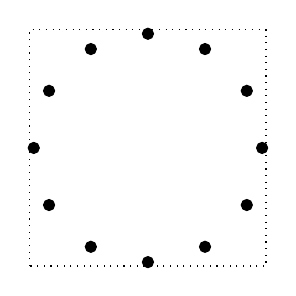
\begin{tikzpicture}
    \draw[thin,dotted] (-1.5,-1.5) rectangle (1.5,1.5);
    \foreach \x in {0,30,...,330} {
        \draw[fill] (\x:1.45cm) circle (2pt);
    }
\end{tikzpicture}
}

\newcommand{\projectPhotographThree}{
\begin{tikzpicture}
    \draw[thin,dotted] (-1.5,-1.5) rectangle (1.5,1.5);
    \foreach \x in {-1.5,-1.0,-0.5,0,0.5,1.0,1.5} {
        \draw[fill] (\x,{1.45-1.30*\x*\x}) circle (2pt);
    }
\end{tikzpicture}
}

\element{project}{
\begin{questionmult}{testA-Q07}
    The following figures represent stroboscopic photographs of a moving ball.
    The strobe rate is constant and is the same for all three ``photographs.''
    %% almost the same as testC-Q24
    Which of the photographs could be produced with a stationary ball and a moving camera?
    %and a camera moving with constant velocity?
    \begin{multicols}{2}
    \begin{choices}
        \AMCboxDimensions{down=-1.5cm}
      \correctchoice{\projectPhotographOne}
      \correctchoice{\projectPhotographTwo}
      \correctchoice{\projectPhotographThree}
        %% NOTE: make a forth for symmetry??
    \end{choices}
    \end{multicols}
\end{questionmult}
}

%% NOTE: testA-Q07 and Q08
%% NOTE: testB-Q01 and Q02
%% NOTE: TODO: complex functions
\newcommand{\projectDistanceFromStartGraph}{
\begin{tikzpicture}
    \begin{axis}[
        axis y line=left,
        axis x line=bottom,
        axis line style={->},
        xlabel={Time from start},
        x unit=\si{\second},
        xtick={0,5,10,15},
        minor x tick num=1,
        xticklabels={127,128,129},
        ylabel={Distance from start},
        y unit=\si{\meter},
        ytick={0,5,10,15},
        minor y tick num=4,
        yticklabels={785,790,795,800},
        xmin=0,xmax=11,
        ymin=0,ymax=16,
        width=1.0\columnwidth,
        height=1.0\columnwidth,
        very thin,
        grid=major,
        clip=false,
        colormap={mymap}{rgb=(0,0,0); rgb=(0,0,0)}
    ]
    %% Line A, B, C, D, E
    %% node[pos=1.0, anchor=west]
    %\addplot[line width=1pt,domain=0:10] {x};
    %% Add A: pos=0.00, B: pos=0.50, C: pos=1.00
    %% Curved lines
    \addplot[line width=1pt,black,draw=black,color=black,patch,patch type=cubic spline]
        coordinates { (0,0) (10,9) (4,3) (7,7) };
    \addplot[line width=1pt,black,draw=black,color=black,patch,patch type=quadratic spline]
        coordinates { (0,2) (10,7) (7,4) };
    \addplot[line width=1pt,black,draw=black,color=black,patch,patch type=cubic spline]
        coordinates { (0,5) (10,14) (3,7) (7,9) };
    \addplot[line width=1pt,black,draw=black,color=black,patch,patch type=quadratic spline]
        coordinates { (0,7) (10,11) (5,10) };
    %% Straight lines
    %\addplot[line width=1pt,black,draw=black,color=black,mark=\empty]
    %    coordinates { (0,7) (10,11) };
    \addplot[line width=1pt,black,draw=black,color=black,mark=\empty]
        coordinates { (0,3) (10,6) };
    %% Nodes on far right edge
    \node[anchor=west] at (axis cs:10,14) {$A$};
    \node[anchor=west] at (axis cs:10,11) {$B$};
    \node[anchor=west] at (axis cs:10,9) {$C$};
    \node[anchor=west] at (axis cs:10,7) {$D$};
    \node[anchor=west] at (axis cs:10,6) {$E$};
    \end{axis}
\end{tikzpicture}
}

\element{project}{
\begin{question}{testA-Q08}
    %Questions 8 and 9 refer to the graph at the right and statement below.
    The graph shows the positions of five sprinters near the end of an \SI{800}{\meter} race.
    \begin{center}
        \projectDistanceFromStartGraph
    \end{center}
    The average speed of sprinter $C$ in the time period
        \SI{127}{\second} to \SI{129}{\second} from the start was approximately
    \begin{multicols}{2}
    \begin{choices}
        %% NOTE: Changed graph for readability
      \correctchoice{\SI{4.5}{\meter\per\second}}
        \wrongchoice{\SI{6.5}{\meter\per\second}}
        \wrongchoice{\SI{8}{\meter\per\second}}
        \wrongchoice{\SI{9}{\meter\per\second}}
        \wrongchoice{\SI{13}{\meter\per\second}}
        %% NOTE: added for symmetry
        \wrongchoice{\SI{11}{\meter\per\second}}
    \end{choices}
    \end{multicols}
\end{question}
}

\element{project}{
\begin{question}{testA-Q09}
    %Questions 8 and 9 refer to the graph at the right and statement below.
    The graph shows the positions of five sprinters near the end of an 800-meter race.
    \begin{center}
        \projectDistanceFromStartGraph
    \end{center}
    Which sprinter runs with uniform speed during the time period shown?
    \begin{multicols}{2}
    \begin{choices}
        \wrongchoice{sprinter $A$}
        \wrongchoice{sprinter $B$}
        \wrongchoice{sprinter $C$}
        \wrongchoice{sprinter $D$}
      \correctchoice{sprinter $E$}
    \end{choices}
    \end{multicols}
\end{question}
}

\element{project}{
\begin{question}{testA-Q10}
    A golf ball is hit toward the pin from a point on the same
        level as the pin and \SI{110}{\yard} away.
    It strikes the ground near the pin.
    Assuming that air resistance had no effect on the ball's path,
        what is the best estimate of the location at which it
        reached the highest point in its path?
    \begin{choices}
        \wrongchoice{within 30 yards of where it was hit}
      \correctchoice{about halfway to the pin}
        \wrongchoice{approximately two-thirds of the way to the pin}
        \wrongchoice{almost directly over the pin}
        \wrongchoice{no estimate is possible. The data are not sufficient for a decision .}
    \end{choices}
\end{question}
}

\newcommand{\projectQuoteEleven}{
    \textsuperscript{1}At 5:01:00 A.M. we activated Rocket Z-4 for \SI{10}{\second}.
    \textsuperscript{2}The thrust gauge showed that the rocket produced a force of \SI{77}{\newton}.
    \textsuperscript{3}Accordingly, we estimated a velocity toward the target vehicle of \SI{4}{\meter\per\second}.
    \textsuperscript{4}We expected to touch the target vehicle in \SI{300}{\second}, at 5:06:10.
    \textsuperscript{5}Actually, we touched at 5:06:28.
}

\element{project}{
\begin{question}{testA-Q11}
    %Questions 11 and 12 refer to the following, which is a
    %    hypothetical report submitted by an astronaut about
    %    a space maneuver intended to link two capsules:
    The following refers to a hypothetical report submitted by an astronaut about a space maneuver intended to link two capsules.
    \emph{Sentences are prefixed with sentence number.}
    \begin{quote}
        \projectQuoteEleven
    \end{quote}
    Which of the sentences above gives the result of a computation
        done by the astronaut that involved the use of Newton's second law?
    \begin{multicols}{2}
    \begin{choices}
        \wrongchoice{1 only}
        \wrongchoice{2 only}
        \wrongchoice{3 only}
      \correctchoice{4 only}
        \wrongchoice{2, 3 and 4 only}
    \end{choices}
    \end{multicols}
\end{question}
}

\element{project}{
\begin{question}{testA-Q12}
    %% make independent
    The following refers to a hypothetical report submitted by an astronaut about a space maneuver intended to link two capsules.
    \emph{Sentences are prefixed with sentence number.}
    \begin{quote}
        \projectQuoteEleven
    \end{quote}
    Which of the sentences above describes how the astronaut
        changed conditions to perform the maneuver?
    \begin{multicols}{2}
    \begin{choices}
      \correctchoice{1 only}
        \wrongchoice{4 only}
        \wrongchoice{5 only}
        \wrongchoice{1 and 4 only}
        \wrongchoice{1 and 5 only}
    \end{choices}
    \end{multicols}
\end{question}
}

\element{project}{
\begin{question}{testA-Q13}
    A child is riding on a merry-go-round, as shown below.
    \begin{center}
    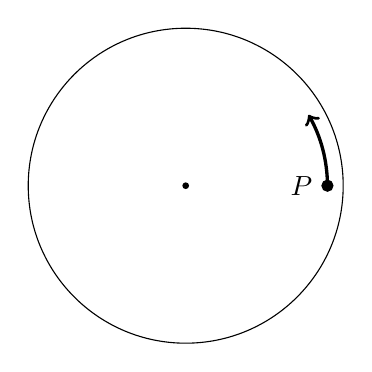
\begin{tikzpicture}
        \draw[fill] circle (1pt);
        \draw[black] circle (2cm);
        \draw[very thick,->] (0:1.8cm) arc (0:30:1.8cm);
        \draw[fill] (0:1.8cm) circle (2pt) node[anchor=east,xshift=-2pt] {$P$};
    \end{tikzpicture}
    \end{center}
    When he is at point $P$,
        which set of vectors shows the direction of his velocity $\vec{v}$,
        his acceleration $\vec{a}$, and the centripetal force $\vec{F}$ acting on him?
    \begin{multicols}{2}
    \begin{choices}
        \AMCboxDimensions{down=-1.5cm}
        \wrongchoice{
            \begin{tikzpicture}
                \draw[thin,dotted] (-1.5,-1.5) rectangle (1.5,1.5);
                \draw[thick,->] (90:2mm) -- ++ (90:1cm)
                    node[pos=0.5,anchor=east] {$\vec{v}$};
                \draw[thick,->] (180:2mm) -- ++ (180:1cm)
                    node[pos=0.5,anchor=north] {$\vec{F}$};
                \draw[thick,->] (0:2mm) -- ++ (0:1cm)
                    node[pos=0.5,anchor=north] {$\vec{a}$};
            \end{tikzpicture}
        }
        \wrongchoice{
            \begin{tikzpicture}
                \draw[thin,dotted] (-1.5,-1.5) rectangle (1.5,1.5);
                \draw[thick,->] (90:2mm) -- ++ (90:1cm)
                    node[pos=0.5,anchor=east] {$\vec{v}$};
                \draw[thick,->] (180:2mm) -- ++ (180:1cm)
                    node[pos=0.5,anchor=north] {$\vec{a}$};
                \draw[thick,->] (270:2mm) -- ++ (270:1cm)
                    node[pos=0.5,anchor=west] {$\vec{F}$};
            \end{tikzpicture}
        }
        \wrongchoice{
            \begin{tikzpicture}
                \draw[thin,dotted] (-1.5,-1.5) rectangle (1.5,1.5);
                \draw[thick,->] (90:2mm) -- ++ (90:1cm)
                    node[pos=0.5,anchor=west] {$\vec{v}$};
                \draw[thick,->] (135:2mm) -- ++ (180:1cm)
                    node[pos=0.5,anchor=south] {$\vec{a}$};
                \draw[thick,->] (225:2mm) -- ++ (180:1cm)
                    node[pos=0.5,anchor=north] {$\vec{F}$};
            \end{tikzpicture}
        }
        \wrongchoice{
            \begin{tikzpicture}
                \draw[thin,dotted] (-1.5,-1.5) rectangle (1.5,1.5);
                \draw[thick,->] (90:2mm) -- ++ (90:1cm)
                    node[pos=0.5,anchor=west] {$\vec{a}$};
                \draw[thick,->] (135:2mm) -- ++ (180:1cm)
                    node[pos=0.5,anchor=south] {$\vec{v}$};
                \draw[thick,->] (225:2mm) -- ++ (180:1cm)
                    node[pos=0.5,anchor=north] {$\vec{F}$};
            \end{tikzpicture}
        }
        \wrongchoice{
            \begin{tikzpicture}
                \draw[thin,dotted] (-1.5,-1.5) rectangle (1.5,1.5);
                \draw[thick,->] (45:2mm) -- ++ (90:1cm)
                    node[pos=0.5,anchor=west] {$\vec{F}$};
                \draw[thick,->] (135:2mm) -- ++ (90:1cm)
                    node[pos=0.5,anchor=east] {$\vec{v}$};
                \draw[thick,->] (180:2mm) -- ++ (180:1cm)
                    node[pos=0.5,anchor=north] {$\vec{a}$};
            \end{tikzpicture}
        }
        %% NOTE: Add sixth for symmetry
        \wrongchoice{
            \begin{tikzpicture}
                \draw[thin,dotted] (-1.5,-1.5) rectangle (1.5,1.5);
                \draw[thick,->] (90:2mm) -- ++ (90:1cm)
                    node[pos=0.5,anchor=east] {$\vec{v}$};
                \draw[thick,->] (180:2mm) -- ++ (180:1cm)
                    node[pos=0.5,anchor=north] {$\vec{F}$};
                \draw[thick,->] (270:2mm) -- ++ (270:1cm)
                    node[pos=0.5,anchor=west] {$\vec{a}$};
            \end{tikzpicture}
        }
    \end{choices}
    \end{multicols}
\end{question}
}

\element{project}{
\begin{question}{testA-Q14}
    A steel ball rolls down an inclined plane.
    Which graph best represents how the distance
        traveled changes with time?
    \begin{multicols}{2}
    \begin{choices}
        \AMCboxDimensions{down=-2.5em}
        \wrongchoice{
            \begin{tikzpicture}
                \begin{axis}[
                    axis y line=left,
                    axis x line=bottom,
                    axis line style={->},
                    xlabel={time},
                    xtick=\empty,
                    ylabel={distance},
                    ytick=\empty,
                    xmin=0,xmax=11,
                    ymin=0,ymax=11,
                    width=1.00\columnwidth,
                    very thin,
                ]
                \addplot[line width=1pt,domain=0:10]{x};
                \end{axis}
            \end{tikzpicture}
        }
        \wrongchoice{
            \begin{tikzpicture}
                \begin{axis}[
                    axis y line=left,
                    axis x line=bottom,
                    axis line style={->},
                    xlabel={time},
                    xtick=\empty,
                    ylabel={distance},
                    ytick=\empty,
                    xmin=0,xmax=11,
                    ymin=0,ymax=11,
                    width=1.00\columnwidth,
                    very thin,
                ]
                \addplot[line width=1pt,domain=0:10]{8};
                \end{axis}
            \end{tikzpicture}
        }
        \wrongchoice{
            \begin{tikzpicture}
                \begin{axis}[
                    axis y line=left,
                    axis x line=bottom,
                    axis line style={->},
                    xlabel={time},
                    xtick=\empty,
                    ylabel={distance},
                    ytick=\empty,
                    xmin=0,xmax=11,
                    ymin=0,ymax=11,
                    width=1.00\columnwidth,
                    very thin,
                ]
                \addplot[line width=1pt,domain=0:10]{10-x};
                \end{axis}
            \end{tikzpicture}
        }
        %% NOTE: constant positive acceleration graph
        \correctchoice{
            \begin{tikzpicture}
                \begin{axis}[
                    axis y line=left,
                    axis x line=bottom,
                    axis line style={->},
                    xlabel={time},
                    xtick=\empty,
                    ylabel={distance},
                    ytick=\empty,
                    xmin=0,xmax=11,
                    ymin=0,ymax=11,
                    width=1.00\columnwidth,
                    very thin,
                ]
                \addplot[line width=1pt,domain=0:10]{0.1*x*x};
                \end{axis}
            \end{tikzpicture}
        }
        \wrongchoice{
            \begin{tikzpicture}
                \begin{axis}[
                    axis y line=left,
                    axis x line=bottom,
                    axis line style={->},
                    xlabel={time},
                    xtick=\empty,
                    ylabel={distance},
                    ytick=\empty,
                    xmin=0,xmax=11,
                    ymin=0,ymax=11,
                    width=1.00\columnwidth,
                    very thin,
                ]
                \addplot[line width=1pt,domain=0:10]{10-(0.1*(x-10)*(x-10))};
                \end{axis}
            \end{tikzpicture}
        }
        %% NOTE: add sixth for symmetry
        \wrongchoice{
            \begin{tikzpicture}
                \begin{axis}[
                    axis y line=left,
                    axis x line=bottom,
                    axis line style={->},
                    xlabel={time},
                    xtick=\empty,
                    ylabel={acceleration},
                    ytick=\empty,
                    xmin=0,xmax=11,
                    ymin=0,ymax=11,
                    width=1.00\columnwidth,
                    very thin,
                ]
                \addplot[line width=1pt,domain=0:10]{10-(0.4*(x-5)*(x-5))};
                \end{axis}
            \end{tikzpicture}
        }
    \end{choices}
    \end{multicols}
\end{question}
}

\element{project}{
\begin{question}{testA-Q15}
    A propeller rotates with constant rate.
    If we consider the two ends of the propeller,
        which graph best represents how the magnitude
        of their acceleration changes with time?
    \begin{multicols}{2}
    \begin{choices}
        \AMCboxDimensions{down=-2.5em}
        \wrongchoice{
            \begin{tikzpicture}
                \begin{axis}[
                    axis y line=left,
                    axis x line=bottom,
                    axis line style={->},
                    xlabel={time},
                    xtick=\empty,
                    ylabel={acceleration},
                    ytick=\empty,
                    xmin=0,xmax=11,
                    ymin=0,ymax=11,
                    width=1.00\columnwidth,
                    very thin,
                ]
                \addplot[line width=1pt,domain=0:10]{x};
                \end{axis}
            \end{tikzpicture}
        }
        %% NOTE: constant acceleration, a=\frac{v^2}{R}
        \correctchoice{
            \begin{tikzpicture}
                \begin{axis}[
                    axis y line=left,
                    axis x line=bottom,
                    axis line style={->},
                    xlabel={time},
                    xtick=\empty,
                    ylabel={acceleration},
                    ytick=\empty,
                    xmin=0,xmax=11,
                    ymin=0,ymax=11,
                    width=1.00\columnwidth,
                    very thin,
                ]
                \addplot[line width=1pt,domain=0:10]{8};
                \end{axis}
            \end{tikzpicture}
        }
        \wrongchoice{
            \begin{tikzpicture}
                \begin{axis}[
                    axis y line=left,
                    axis x line=bottom,
                    axis line style={->},
                    xlabel={time},
                    xtick=\empty,
                    ylabel={acceleration},
                    ytick=\empty,
                    xmin=0,xmax=11,
                    ymin=0,ymax=11,
                    width=1.00\columnwidth,
                    very thin,
                ]
                \addplot[line width=1pt,domain=0:10]{10-(0.4*(x-5)*(x-5))};
                \end{axis}
            \end{tikzpicture}
        }
        \wrongchoice{
            \begin{tikzpicture}
                \begin{axis}[
                    axis y line=left,
                    axis x line=bottom,
                    axis line style={->},
                    xlabel={time},
                    xtick=\empty,
                    ylabel={acceleration},
                    ytick=\empty,
                    xmin=0,xmax=11,
                    ymin=0,ymax=11,
                    width=1.00\columnwidth,
                    very thin,
                ]
                \addplot[line width=1pt,domain=0:10]{0.1*x*x};
                \end{axis}
            \end{tikzpicture}
        }
        \wrongchoice{
            \begin{tikzpicture}
                \begin{axis}[
                    axis y line=left,
                    axis x line=bottom,
                    axis line style={->},
                    xlabel={time},
                    xtick=\empty,
                    ylabel={acceleration},
                    ytick=\empty,
                    xmin=0,xmax=11,
                    ymin=0,ymax=11,
                    width=1.00\columnwidth,
                    very thin,
                ]
                \addplot[line width=1pt,domain=0:10]{10-(0.1*(x-10)*(x-10))};
                \end{axis}
            \end{tikzpicture}
        }
        %% NOTE: add sixth for symmetry
        \wrongchoice{
            \begin{tikzpicture}
                \begin{axis}[
                    axis y line=left,
                    axis x line=bottom,
                    axis line style={->},
                    xlabel={time},
                    xtick=\empty,
                    ylabel={acceleration},
                    ytick=\empty,
                    xmin=0,xmax=11,
                    ymin=0,ymax=11,
                    width=1.00\columnwidth,
                    very thin,
                ]
                \addplot[line width=1pt,domain=0:10]{10-x};
                \end{axis}
            \end{tikzpicture}
        }
    \end{choices}
    \end{multicols}
\end{question}
}


%% Test B
%%--------------------
\element{project}{
\begin{question}{testB-Q01}
    Questions 1 and 2 refer to the figure at right,
        which shows the positions of five runners
        near the end of an \SI{800}{\meter} race.
    \begin{center}
        \projectDistanceFromStartGraph
    \end{center}
    Which sprinter was ahead after exactly \SI{127}{\second}?
    \begin{multicols}{2}
    \begin{choices}
        \wrongchoice{sprinter $A$}
      \correctchoice{sprinter $B$}
        \wrongchoice{sprinter $C$}
        \wrongchoice{sprinter $D$}
        \wrongchoice{sprinter $E$}
    \end{choices}
    \end{multicols}
\end{question}
}

\element{project}{
\begin{question}{testB-Q02}
    Questions 1 and 2 refer to the figure at right,
        which shows the positions of five runners
        near the end of an \SI{800}{\meter} race.
    \begin{center}
        \projectDistanceFromStartGraph
    \end{center}
    With what average speed did $E$ run in the interval \SIrange{127}{129}{\second}?
    \begin{multicols}{2}
    \begin{choices}
        %% NOTE: changed graph for readability
        \wrongchoice{\SI{1}{\meter\per\second}}
      \correctchoice{\SI{3}{\meter\per\second}}
        \wrongchoice{\SI{7}{\meter\per\second}}
        \wrongchoice{\SI{9}{\meter\per\second}}
        \wrongchoice{\SI{11}{\meter\per\second}}
        %% NOTE: added for symmetry
        \wrongchoice{\SI{13}{\meter\per\second}}
    \end{choices}
    \end{multicols}
\end{question}
}

\element{project}{
\begin{question}{testB-Q03}
    Which of the following four statements describes the motion
        of a bullet that has been fired by a supersonic jet
        fighter plane flying parallel to the ground?
    (Neglect air resistance.)
    \begin{choices}
        \wrongchoice{uniform straight-line motion}
        \wrongchoice{uniformly accelerated straight-line motion}
        \wrongchoice{circular motion}
      \correctchoice{projectile motion}
    \end{choices}
\end{question}
}

\element{project}{
\begin{question}{testB-Q04}
    Which of the following four diagrams represents the
        acceleration of a golf ball the instant after it
        leaves the face of a golf club?
    \begin{multicols}{2}
    \begin{choices}
        \AMCboxDimensions{down=-0.8cm}
        \correctchoice{
            \begin{tikzpicture}
                \draw[thin,dashed] (-1,0) rectangle (1,-2);
                \draw[fill] (0,0) circle (1.5pt);
                \draw[thick,->] (0,0) -- ++ (270:2cm) node[pos=0.5,anchor=west] {$\vec{a}$};
            \end{tikzpicture}
        }
        \wrongchoice{
            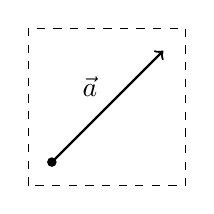
\begin{tikzpicture}
                \draw[thin,dashed] (-0.3,-0.3) rectangle (1.7,1.7);
                \draw[fill] (0,0) circle (1.5pt);
                \draw[thick,->] (0,0) -- ++ (45:2cm) node[pos=0.5,anchor=south east] {$\vec{a}$};
            \end{tikzpicture}
        }
        \wrongchoice{
            \begin{tikzpicture}
                \draw[thin,dashed] (0,-1) rectangle (2,1);
                \draw[fill] (0,0) circle (1.5pt);
                \draw[thick,->] (0,0) -- ++ (0:2cm) node[pos=0.5,anchor=south] {$\vec{a}$};
            \end{tikzpicture}
        }
        \wrongchoice{
            \begin{tikzpicture}
                \draw[thin,dashed] (-1,-1) rectangle (1,1);
                \draw[fill] (0,0) circle (1.5pt)
                    node [anchor=south] {$\vec{a}=0$};
            \end{tikzpicture}
        }
    \end{choices}
    \end{multicols}
\end{question}
}

\element{project}{
\begin{questionmult}{testB-Q05}
    An ice skater gives a sudden push to a sled that sends it sliding away from him.
    Consider the following statements (assume friction is negligible).
    Which of the statements is true if the skater and the sled have the same mass?
    %% NOTE: changed to questionmult
    \begin{choices}
        %% NOTE: answer is ``1 only''
        %% NOTE: third one is tricky to eliminate
      \correctchoice{The force exerted on the sled by the skater is equal in magnitude to the force exerted on the skater by the sled.}
        \wrongchoice{During the push the acceleration of the skater is equal in magnitude to the acceleration of the sled.}
        \wrongchoice{The skater will accelerate for the same length of time as the sled.}
    \end{choices}
\end{questionmult}
}

\element{project}{
\begin{questionmult}{testB-Q06}
    A child is riding on a merry-go-round that is rotating at a constant rate.
    The child has
    %% NOTE: changed to questionmult
    \begin{choices}
        \wrongchoice{constant velocity.}
        \wrongchoice{constant acceleration.}
      \correctchoice{constant speed.}
    \end{choices}
\end{questionmult}
}

\element{project}{
\begin{question}{testB-Q07}
    %% reworded question
    %In the graph below,
    The velocity of an object is represented graphically below.
    \begin{center}
        \projectSpeedGraph{velocity}
    \end{center}
    The magnitude of the acceleration is greatest in the time interval:
    \begin{multicols}{3}
    \begin{choices}
        \wrongchoice{$a$ to $c$}
        \wrongchoice{$c$ to $e$}
        \wrongchoice{$e$ to $g$}
      \correctchoice{$g$ to $i$}
        \wrongchoice{$i$ to $k$}
    \end{choices}
    \end{multicols}
\end{question}
}

\element{project}{
\begin{question}{testB-Q08}
    \emph{All except one} of the following require a net unbalanced force.
    Which is the exception?
    \begin{choices}
        \wrongchoice{to set into motion an object which is initially at rest.}
      \correctchoice{to maintain an object in a state of constant velocity.}
        \wrongchoice{to maintain an object in a state of uniform circular motion.}
        \wrongchoice{to stop a moving object.}
        \wrongchoice{to change an object's direction of motion while keeping its speed constant.}
    \end{choices}
\end{question}
}

\element{project}{
\begin{question}{testB-Q09}
    The distance $d$ traveled by an object is given by the
        equation $d=\dfrac{1}{2}at^2$, when the object
    \begin{choices}
        \wrongchoice{is moving in a circle.}
        \wrongchoice{has a constant velocity.}
      \correctchoice{starts from rest and accelerates uniformly.}
        \wrongchoice{is thrown upward.}
        \wrongchoice{is thrown downward.}
    \end{choices}
\end{question}
}

\element{project}{
\begin{question}{testB-Q10}
    This test paper is sitting at rest on your desk.
    Which of the following statements best describes this situation?
    \begin{choices}
        \wrongchoice{There are no forces acting on your paper.}
        \wrongchoice{Your paper is at rest in any coordinate system.}
        \wrongchoice{Your paper exerts no force on the desk.}
      \correctchoice{There are many forces acting on your paper, but they balance each other.}
    \end{choices}
\end{question}
}

\element{project}{
\begin{question}{testB-Q11}
    A satellite is in orbit around the earth,
        in the absence of air friction,
        which of the following statements is necessarily true?
    \begin{choices}
        \wrongchoice{The acceleration and velocity of the
            satellite are in approximately the same direction.}
        \wrongchoice{There is no force acting on the satellite.}
        \wrongchoice{The velocity of the satellite is constant.}
        \wrongchoice{The satellite must fall back to earth when its fuel is gone.}
      \correctchoice{The satellite always accelerates towards the earth.}
    \end{choices}
\end{question}
}

\element{project}{
\begin{question}{testB-Q12}
    If you must choose between two hypotheses,
        which of the following is the best reason for
        selecting hypothesis 1 rather than hypothesis 2?
    \begin{choices}
      \correctchoice{Hypothesis 1 is more in agreement with the observed facts.}
        \wrongchoice{Hypothesis 1 contains more mathematics.}
        \wrongchoice{Hypothesis 1 is newer.}
        \wrongchoice{Hypothesis 1 is more easily understood.}
        \wrongchoice{Several people think hypothesis 1 is more likely to be correct.}
    \end{choices}
\end{question}
}

\element{project}{
\begin{question}{testB-Q13}
    A rock is thrown into the air.
    Which graph represents how the magnitude of its acceleration
        changes with time while it is in the air?
    (Neglect air resistance.)
    \begin{multicols}{2}
    \begin{choices}
        \AMCboxDimensions{down=-2.5em}
        \wrongchoice{
            \begin{tikzpicture}
                \begin{axis}[
                    axis y line=left,
                    axis x line=bottom,
                    axis line style={->},
                    xlabel={time},
                    xtick=\empty,
                    ylabel={acceleration},
                    ytick=\empty,
                    xmin=0,xmax=11,
                    ymin=0,ymax=11,
                    width=1.00\columnwidth,
                    very thin,
                ]
                \addplot[line width=1pt,domain=0:10]{x};
                \end{axis}
            \end{tikzpicture}
        }
        %% NOTE: gravity is constant
        \correctchoice{
            \begin{tikzpicture}
                \begin{axis}[
                    axis y line=left,
                    axis x line=bottom,
                    axis line style={->},
                    xlabel={time},
                    xtick=\empty,
                    ylabel={acceleration},
                    ytick=\empty,
                    xmin=0,xmax=11,
                    ymin=0,ymax=11,
                    width=1.00\columnwidth,
                    very thin,
                ]
                \addplot[line width=1pt,domain=0:10]{8};
                \end{axis}
            \end{tikzpicture}
        }
        \wrongchoice{
            \begin{tikzpicture}
                \begin{axis}[
                    axis y line=left,
                    axis x line=bottom,
                    axis line style={->},
                    xlabel={time},
                    xtick=\empty,
                    ylabel={acceleration},
                    ytick=\empty,
                    xmin=0,xmax=11,
                    ymin=0,ymax=11,
                    width=1.00\columnwidth,
                    very thin,
                ]
                \addplot[line width=1pt,domain=0:10]{0.4*x*(x-10)};
                \end{axis}
            \end{tikzpicture}
        }
        \wrongchoice{
            \begin{tikzpicture}
                \begin{axis}[
                    axis y line=left,
                    axis x line=bottom,
                    axis line style={->},
                    xlabel={time},
                    xtick=\empty,
                    ylabel={acceleration},
                    ytick=\empty,
                    xmin=0,xmax=11,
                    ymin=0,ymax=11,
                    width=1.00\columnwidth,
                    very thin,
                ]
                \addplot[line width=1pt,domain=0:10]{0.1*x*x};
                \end{axis}
            \end{tikzpicture}
        }
        \wrongchoice{
            \begin{tikzpicture}
                \begin{axis}[
                    axis y line=left,
                    axis x line=bottom,
                    axis line style={->},
                    xlabel={time},
                    xtick=\empty,
                    ylabel={acceleration},
                    ytick=\empty,
                    xmin=0,xmax=11,
                    ymin=0,ymax=11,
                    width=1.00\columnwidth,
                    very thin,
                ]
                %\addplot[line width=1pt,domain=0:10]{10-(0.1*(x-10)*(x-10))};
                \addplot[line width=1pt,domain=0:10]{3.16 * sqrt(x)};
                \end{axis}
            \end{tikzpicture}
        }
        %% NOTE: add one for symmetry
        \wrongchoice{
            \begin{tikzpicture}
                \begin{axis}[
                    axis y line=left,
                    axis x line=bottom,
                    axis line style={->},
                    xlabel={time},
                    xtick=\empty,
                    ylabel={acceleration},
                    ytick=\empty,
                    xmin=0,xmax=11,
                    ymin=0,ymax=11,
                    width=1.00\columnwidth,
                    very thin,
                ]
                \addplot[line width=1pt,domain=0:10]{10/x};
                \end{axis}
            \end{tikzpicture}
        }
    \end{choices}
    \end{multicols}
\end{question}
}

\element{project}{
\begin{question}{testB-Q14}
    A propeller blade rotates at a constant rate.
    Which graph best represents how the magnitude of the
        force on one tip of the propeller changes with time?
    \begin{multicols}{2}
    \begin{choices}
        \AMCboxDimensions{down=-2.5em}
        \wrongchoice{
            \begin{tikzpicture}
                \begin{axis}[
                    axis y line=left,
                    axis x line=bottom,
                    axis line style={->},
                    xlabel={time},
                    xtick=\empty,
                    ylabel={force},
                    ytick=\empty,
                    xmin=0,xmax=11,
                    ymin=0,ymax=11,
                    width=1.00\columnwidth,
                    very thin,
                ]
                \addplot[line width=1pt,domain=0:10]{x};
                \end{axis}
            \end{tikzpicture}
        }
        %% NOTE: centripetal force is constant
        \correctchoice{
            \begin{tikzpicture}
                \begin{axis}[
                    axis y line=left,
                    axis x line=bottom,
                    axis line style={->},
                    xlabel={time},
                    xtick=\empty,
                    ylabel={force},
                    ytick=\empty,
                    xmin=0,xmax=11,
                    ymin=0,ymax=11,
                    width=1.00\columnwidth,
                    very thin,
                ]
                \addplot[line width=1pt,domain=0:10]{8};
                \end{axis}
            \end{tikzpicture}
        }
        \wrongchoice{
            \begin{tikzpicture}
                \begin{axis}[
                    axis y line=left,
                    axis x line=bottom,
                    axis line style={->},
                    xlabel={time},
                    xtick=\empty,
                    ylabel={force},
                    ytick=\empty,
                    xmin=0,xmax=11,
                    ymin=0,ymax=11,
                    width=1.00\columnwidth,
                    very thin,
                ]
                \addplot[line width=1pt,domain=0:10]{10/x};
                \end{axis}
            \end{tikzpicture}
        }
        \wrongchoice{
            \begin{tikzpicture}
                \begin{axis}[
                    axis y line=left,
                    axis x line=bottom,
                    axis line style={->},
                    xlabel={time},
                    xtick=\empty,
                    ylabel={force},
                    ytick=\empty,
                    xmin=0,xmax=11,
                    ymin=0,ymax=11,
                    width=1.00\columnwidth,
                    very thin,
                ]
                \addplot[line width=1pt,domain=0:10]{0.1*x*x};
                \end{axis}
            \end{tikzpicture}
        }
        \wrongchoice{
            \begin{tikzpicture}
                \begin{axis}[
                    axis y line=left,
                    axis x line=bottom,
                    axis line style={->},
                    xlabel={time},
                    xtick=\empty,
                    ylabel={force},
                    ytick=\empty,
                    xmin=0,xmax=11,
                    ymin=0,ymax=11,
                    width=1.00\columnwidth,
                    very thin,
                ]
                %\addplot[line width=1pt,domain=0:10]{10-(0.1*(x-10)*(x-10))};
                \addplot[line width=1pt,domain=0:10]{3.16 * sqrt(10)};
                \end{axis}
            \end{tikzpicture}
        }
        %% NOTE: add one for symmetry
        \wrongchoice{
            \begin{tikzpicture}
                \begin{axis}[
                    axis y line=left,
                    axis x line=bottom,
                    axis line style={->},
                    xlabel={time},
                    xtick=\empty,
                    ylabel={force},
                    ytick=\empty,
                    xmin=0,xmax=11,
                    ymin=0,ymax=11,
                    width=1.00\columnwidth,
                    very thin,
                ]
                \addplot[line width=1pt,domain=0:10]{10-x};
                \end{axis}
            \end{tikzpicture}
        }
    \end{choices}
    \end{multicols}
\end{question}
}

\element{project}{
\begin{question}{testB-Q15}
    In the diagrams shown below, arrows show the direction
        of the velocity and acceleration vectors for a car
        at five separate instants of time.
    Which diagram represents the car starting from rest?
    \begin{multicols}{2}
    \begin{choices}
        \AMCboxDimensions{down=-2.0cm}
        \wrongchoice{
            \begin{tikzpicture}
                \draw[thin,dotted] (-1.5,-2) rectangle (1.5,2);
                \draw[thick,->] (-1,1) -- (1,1)
                    node[pos=0.5,anchor=south] {$\vec{v}$};
                \draw[thick,->] (0,-1.5) -- (0,0.5)
                    node[pos=0.5,anchor=west] {$\vec{a}$};
            \end{tikzpicture}
        }
        \wrongchoice{
            \begin{tikzpicture}
                \draw[thin,dotted] (-1.5,-2) rectangle (1.5,2);
                \draw[thick,->] (-1,0.5) -- (1,0.5)
                    node[pos=0.5,anchor=south] {$\vec{v}$};
                \draw[thick,->] (-0.8,-0.5) -- (0.8,-0.5)
                    node[pos=0.5,anchor=south] {$\vec{a}$};
            \end{tikzpicture}
        }
        \wrongchoice{
            \begin{tikzpicture}
                \draw[thin,dotted] (-1.5,-2) rectangle (1.5,2);
                \draw[thick,->] (-1,0.5) -- (1,0.5)
                    node[pos=0.5,anchor=south] {$\vec{v}$};
                \draw[thick,<-] (-0.8,-0.5) -- (0.8,-0.5)
                    node[pos=0.5,anchor=south] {$\vec{a}$};
            \end{tikzpicture}
        }
        \wrongchoice{
            \begin{tikzpicture}
                \draw[thin,dotted] (-1.5,-2) rectangle (1.5,2);
                \draw[thick,->] (-1,0.5) -- (1,0.5)
                    node[pos=0.5,anchor=south] {$\vec{v}$};
                \draw[fill] (0,-0.5) circle (2pt);
                \node[anchor=south] at (0,-0.5) {$\vec{a}=0$};
            \end{tikzpicture}
        }
        %% NOTE: v=0
        \correctchoice{
            \begin{tikzpicture}
                \draw[thin,dotted] (-1.5,-2) rectangle (1.5,2);
                \draw[fill] (0,0.5) circle (2pt);
                \node[anchor=south] at (0,0.5) {$\vec{v}=0$};
                \draw[thick,<-] (-0.8,-0.5) -- (0.8,-0.5)
                    node[pos=0.5,anchor=south] {$\vec{a}$};
            \end{tikzpicture}
        }
        %% NOTE: add one for symmetry
    \end{choices}
    \end{multicols}
\end{question}
}


%% Test C
%%--------------------
\element{project}{
\begin{question}{testC-Q01}
    An experiment yielded the data given in the table and graph below.
    \begin{center}
    ~\hspace{1em}
    \begin{tabular}{lcccc}
        \toprule
        $t$ [\si{\second}] &
            0 & 2 & 4 & 6 \\
        $d$ [\si{\meter}] &
            0 & 4 & 8 & 12 \\
        \bottomrule
    \end{tabular}
    \vspace{2.0\baselineskip}
    \begin{tikzpicture}
        \begin{axis}[
            axis y line=left,
            axis x line=bottom,
            axis line style={->},
            xlabel={$t$},
            x unit=\si{\second},
            xtick={0,2,4,6},
            ylabel={$d$},
            y unit=\si{\meter},
            ytick={0,4,8,12},
            minor y tick num=1,
            xmin=0,xmax=6.5,
            ymin=0,ymax=13,
            width=0.8\columnwidth,
            height=0.5\columnwidth,
            very thin,
        ]
        \addplot[only marks,mark=*,mark size=2pt] coordinates {(0,0) (2,4) (4,8) (6,12)};
        \end{axis}
    \end{tikzpicture}
    \end{center}
    If these data are expressed as an equation,
        $d = kt$, the value of $k$ is:
    \begin{multicols}{3}
    \begin{choices}
        \wrongchoice{\SI{1}{\meter\per\second}}
        \wrongchoice{\SI{1}{\second\per\meter}}
      \correctchoice{\SI{2}{\meter\per\second}}
        \wrongchoice{\SI{2}{\second\per\meter}}
        \wrongchoice{\SI{0.5}{\meter\per\second}}
        %% NOTE: for symmetry
        \wrongchoice{\SI{0.5}{\second\per\meter}}
    \end{choices}
    \end{multicols}
\end{question}
}

\element{project}{
\begin{question}{testC-Q02}
    Referring to his work, Newton wrote,
        ``If I have seen further than others,
        it is because I have stood on the shoulders of giants.''
    Who of the following was one of the ``giants''
        whose work on motion immediately preceded Newton's?
    \begin{multicols}{2}
    \begin{choices}
        \wrongchoice{Fermi}
      \correctchoice{Galileo}
        \wrongchoice{Simplicio}
        \wrongchoice{Aristotle}
    \end{choices}
    \end{multicols}
\end{question}
}

\element{project}{
\begin{question}{testC-Q03}
    The arrows drawn below represent the velocity vectors of a
        Boeing 707 jet at three successive times.
    %% foreach x/y {1/90, 1/45, 3/0}
    %% forward and backwards to keep centered
    \begin{center}
    \begin{tikzpicture}
        \draw[very thick,->] (0,0) -- ++ (90:1.5cm)
            node[pos=0,anchor=north] {$t_1:$};
        \draw[very thick,->] (1.5,0) -- ++ (45:1.5cm)
            node[pos=0,anchor=north] {$t_2:$};
        \draw[very thick,->] (3.0,0) -- ++ (0:1.5cm)
            node[pos=0,anchor=north east] {$t_3:$};
    \end{tikzpicture}
    \end{center}
    We may conclude that the jet was
    \begin{choices}
      \correctchoice{changing direction.}
        \wrongchoice{speeding up.}
        \wrongchoice{slowing down.}
        \wrongchoice{maintaining a constant velocity.}
    \end{choices}
\end{question}
}

\newcommand{\tbONEexCqZeroFour}{
\begin{tikzpicture}
    \begin{axis}[
        axis y line=left,
        axis x line=bottom,
        axis line style={->},
        ylabel={Total distance traversed},
        y unit=\si{\meter},
        ytick={0.02,0.04,0.06},
        ymin=0,ymax=0.07,
        xlabel={Total elapsed time},
        x unit=\si{\second},
        xtick={1,2,3,4,5,6,7,8},
        xticklabels={$t_1$,$t_2$,$t_3$,$t_4$,$t_5$,$t_6$,$t_7$,$t_8$},
        xmin=0,xmax=9,
        width=0.95\columnwidth,
        height=0.618\columnwidth,
        very thin,
    ]
    \addplot[dashed,line width=1pt,domain=0:9] {0.00083*x*x};
    \draw[fill] (axis cs:2,0.0033) circle (1.5pt) node[anchor=south] {$P_2$};
    \draw[fill] (axis cs:4,0.0133) circle (1.5pt) node[anchor=south] {$P_4$};
    \draw[fill] (axis cs:6,0.0300) circle (1.5pt) node[anchor=south] {$P_6$};
    \end{axis}
\end{tikzpicture}
}

\element{project}{
\begin{question}{testC-Q04}
    %Questions 4 and 5 refer to the following statement and graph:
    The graph below shows the relationship between the
        time and the total distance traversed by a glider moving
        on a nearly frictionless air track.
    Points $P_2$, $P_4$ and $P_6$ represent the experimental measurements.
    The dotted curve is a smooth curve drawn through these points.
    \begin{center}
        \tbONEexCqZeroFour
    \end{center}
    If the values of the total distance traversed at times
        $t_5$, $t_6$ and $t_8$ are arranged in order of
        uncertainty with the most \emph{uncertain} value of
        distance first, the order is
    \begin{multicols}{2}
    \begin{choices}
        \wrongchoice{$t_5$, $t_6$, $t_8$.}
        \wrongchoice{$t_8$, $t_6$, $t_5$.}
        \wrongchoice{$t_5$, $t_8$, $t_6$.}
        \wrongchoice{$t_6$, $t_5$, $t_8$.}
        %% NOTE: t_8 is extrapolation
        %% NOTE: t_5 is interpolation
        %% NOTE: t_6 is a data point
      \correctchoice{$t_8$, $t_5$, $t_6$.}
    \end{choices}
    \end{multicols}
\end{question}
}

\element{project}{
\begin{question}{testC-Q05}
    %% NOTE: change wording
    Questions 4 and 5 refer to the following statement and graph:
        The graph at the right shows the relationship between the
        time and the total distance traversed by a glider moving
        on a nearly frictionless air track.
    Points $P_2$, $P_4$ and $P_6$ represent the experimental measurements.
    The dotted curve is a smooth curve drawn through these points.
    \begin{center}
        \tbONEexCqZeroFour
    \end{center}
    The slope of the curve at $t_4$ represents the
    \begin{choices}
        \wrongchoice{total distance traversed.}
      \correctchoice{instantaneous speed.}
        \wrongchoice{acceleration.}
        \wrongchoice{rates of change of speed.}
        \wrongchoice{average speed.}
    \end{choices}
\end{question}
}

\element{project}{
\begin{question}{testC-Q06}
    Two men push on a box resting on a smooth level floor
        as indicated in the diagram below.
    The lengths of the arrows are drawn proportional to the
        magnitude of the force each man exerts on the box.
    %% Reword question more generally, or abstractly
    \begin{center}
    \begin{tikzpicture}
        \draw (0,0) rectangle (2,2);
        %% NOTE: 3 * tan(30) = 1.44
        \draw[thick,->] (1,1) -- ++ (90:1.44);
        \draw[thick,->] (1,1) -- ++ (0:3);
    \end{tikzpicture}
    \end{center}
    In the diagrams below,
        which arrow indicates the direction in which the box will start to move?
    \begin{multicols}{2}
    \begin{choices}
        %% NOTE: go backwards then forward to keep vector centered in option
        \AMCboxDimensions{down=-1cm}
        \wrongchoice{
            \begin{tikzpicture}
                \draw[thin,dashed] (-0.15,-0.15) rectangle (1.5,1.5);
                \draw[thick,->] (0,0) -- ++ (90:1.45cm);
            \end{tikzpicture}
        }
        \wrongchoice{
            \begin{tikzpicture}
                \draw[thin,dashed] (-0.15,-0.15) rectangle (1.5,1.5);
                \draw[thick,->] (0,0) -- ++ (60:1.45cm);
            \end{tikzpicture}
        }
        \wrongchoice{
            \begin{tikzpicture}
                \draw[thin,dashed] (-0.15,-0.15) rectangle (1.5,1.5);
                \draw[thick,->] (0,0) -- ++ (45:1.45cm);
            \end{tikzpicture}
        }
        %% NOTE: horizontal is bigger than vertical
        \correctchoice{
            \begin{tikzpicture}
                \draw[thin,dashed] (-0.15,-0.15) rectangle (1.5,1.5);
                \draw[thick,->] (0,0) -- ++ (30:1.45cm);
            \end{tikzpicture}
        }
        \wrongchoice{
            \begin{tikzpicture}
                \draw[thin,dashed] (-0.15,-0.15) rectangle (1.5,1.5);
                \draw[thick,->] (0,0) -- ++ (0:1.45cm);
            \end{tikzpicture}
        }
    \end{choices}
    \end{multicols}
\end{question}
}

\element{project}{
\begin{question}{testC-Q07}
    A satellite is in a circular orbit around a planet.
    The satellite's period of revolution $T$,
        and the radius of the orbit $R$ are known.
    Which of the following equations must you use to compute its acceleration?
    \begin{choices}
        \wrongchoice{$d=\dfrac{1}{2} aT^2$ only.}
        \wrongchoice{$v=\dfrac{2\pi R}{T}$ and $v=aT$.}
      \correctchoice{$v=\dfrac{2\pi R}{T}$ and $a=\dfrac{v^2}{R}$.}
        \wrongchoice{$d=\dfrac{1}{2}aT$ and $a=\dfrac{v^2}{R}$.}
        \wrongchoice{$v=aT$ and $a=\dfrac{v^2}{R}$.}
    \end{choices}
\end{question}
}

\element{project}{
\begin{question}{testC-Q08}
    A man pushes a puck on a frictionless horizontal
        surface with a force of \SI{10}{\newton}.
    The resulting acceleration is \SI{4.0}{\meter\per\second\squared}.
    What is the mass of the puck?
    \begin{multicols}{3}
    \begin{choices}
        \wrongchoice{\SI{0.4}{\kilo\gram}}
      \correctchoice{\SI{2.5}{\kilo\gram}}
        \wrongchoice{\SI{4.0}{\kilo\gram}}
        \wrongchoice{\SI{10}{\kilo\gram}}
        \wrongchoice{\SI{40}{\kilo\gram}}
        %% NOTE: add one for symmetry
        \wrongchoice{\SI{14}{\kilo\gram}}
    \end{choices}
    \end{multicols}
\end{question}
}

%\element{project}{
%\begin{question}{testC-Q09}
%    The diagram at right shows a cable car supported by an
%        overhead cable and pulled uphill by a second cable.
%    \begin{center}
%    \begin{tikzpicture}
%        %% NOTE: TODO: diagram
%    \end{tikzpicture}
%    \end{center}
%    Which of the following forces is zero when the cable
%        car moves with constant velocity?
%    \begin{choices}
%      \correctchoice{net unbalanced force on the car and carriage}
%        \wrongchoice{frictional force on the wheels of the carriage}
%        \wrongchoice{force of gravity on the car and carriage}
%        \wrongchoice{force exerted by supporting cables}
%        \wrongchoice{force exerted by the cable that pulls the car upward}
%    \end{choices}
%\end{question}
%}

\element{project}{
\begin{question}{testC-Q10}
    In \emph{all except one} of the following situations,
        an object is being accelerated.
    Which one is the exception?
    \begin{choices}
        \wrongchoice{The object changes direction without changing speed.}
        \wrongchoice{The object changes speed without changing direction.}
      \correctchoice{The object maintains speed and direction.}
        \wrongchoice{The object maintains uniform circular motion.}
        \wrongchoice{The object moves in the trajectory of a projectile.}
    \end{choices}
\end{question}
}

\element{project}{
\begin{question}{testC-Q11}
    %Questions 11 and 12 refer to the following situation.
    During a planned maneuver in space flight, a free-floating astronaut
        pushes a free-floating instrument package.
    The mass of the astronaut is greater than that of the instrument package.

    The force exerted by the astronaut on the instrument package:
    \begin{choices}
      \correctchoice{is equal to the force exerted by the package on the astronaut.}
        \wrongchoice{is greater than the force exerted by the package on the astronaut.}
        \wrongchoice{is less than the force exerted by the package on the astronaut.}
        \wrongchoice{is equal to zero.}
        \wrongchoice{may be greater than, less than, or equal to the force exerted by the package on the astronaut; one cannot tell with the information given here.}
    \end{choices}
\end{question}
}

\element{project}{
\begin{question}{testC-Q12}
    %Questions 11 and 12 refer to the following situation.
    During a planned maneuver in space flight, a free-floating astronaut
        pushes a free-floating instrument package.
    The mass of the astronaut is greater than that of the instrument package.

    During the push:
    \begin{choices}
        \wrongchoice{the magnitude of the acceleration of the astronaut is greater than that of the instrument package.}
      \correctchoice{the magnitude of the acceleration of the astronaut is smaller than that of the instrument package.}
        \wrongchoice{neither astronaut nor instrument package is accelerated.}
        \wrongchoice{the accelerations of each are equal in magnitude but opposite in direction.}
        \wrongchoice{the accelerations of each are equal in magnitude and in the same direction.}
    \end{choices}
\end{question}
}

\element{project}{
\begin{question}{testC-Q13}
    In Two New Sciences Salviati, speaking for Galileo, defines
        ``a motion to be uniformly accelerated, when starting
        from rest it acquires during equal time intervals, equal increments of speed.''
    This definition is important because it
    \begin{choices}
        \wrongchoice{convinces Simplicio, the spokesman for Aristotelian physics.}
      \correctchoice{corresponds closely to the way real objects fall near the surface of the earth.}
        \wrongchoice{explains the cause of acceleration of falling objects.}
        \wrongchoice{is correct regardless of the air resistance of falling objects.}
        \wrongchoice{is the only definition that can be tested by experiment.}
    \end{choices}
\end{question}
}

\element{project}{
\begin{question}{testC-Q14}
    \emph{All except one} of the following statements would be
        operational definitions of one second of time.
    Which one is the exception? \\[-0.5\baselineskip]
    %% start question
    One second is:
    \begin{choices}
        \wrongchoice{a little more time than there is between the pulsebeats of most people.}
        %% NOTE: not an operational definition
      \correctchoice{the shortest unit of time.}
        \wrongchoice{$\dfrac{1}{86\,400}$ of the time it takes the earth to make one rotation about its axis.}
        \wrongchoice{the length of a time interval a little shorter than it takes a student to answer this question.}
    \end{choices}
\end{question}
}

\element{project}{
\begin{question}{testC-Q15}
    %Questions 15 and 16 refer to the following statement.
    Scientists on the imaginary planet $Q$ have defined a unit of length,
        the ``lar,'' to be the distance between two mountain
        peaks on the surface of the planet.
    The unit of time on the planet $Q$ is called the ``tik''
        and is defined as the average interval between
        pulsebeats of the king. \\[-0.5\baselineskip]
    %% start question
    What units would express acceleration on planet $Q$
        if acceleration were defined as it is on earth?
    \begin{multicols}{2}
    \begin{choices}
        \wrongchoice{\si{lar\per{}tik}}
        \wrongchoice{\si{lar\per\second}}
        \wrongchoice{\si{lar\squared\per\second}}
        \wrongchoice{\si{tik\per{}lar\squared}}
      \correctchoice{\si{lar\per{}tik\squared}}
      %% NOTE: symmetry
        \wrongchoice{\si{tik\per\second\squared}}
    \end{choices}
    \end{multicols}
\end{question}
}

\element{project}{
\begin{question}{testC-Q16}
    %Questions 15 and 16 refer to the following statement.
    Scientists on the imaginary planet $Q$ have defined a unit of length,
        the ``lar,'' to be the distance between two mountain
        peaks on the surface of the planet.
    The unit of time on the planet $Q$ is called the ``tik''
        and is defined as the average interval between
        pulsebeats of the king. \\[-0.5\baselineskip]
    %% start question
    If the distance between the cities Zytropolis and Elany on
        planet $Q$ is \SI{20}{lar}, what would your average speed
        be if you made the trip in \SI{100}{tik}?
    \begin{multicols}{2}
    \begin{choices}
      \correctchoice{\SI{0.2}{lar\per{}tik}}
        \wrongchoice{\SI{0.1}{tik\per{}lar}}
        \wrongchoice{\SI{5}{tik\per{}lar}}
        \wrongchoice{\SI{5}{lar\per{}tik}}
        \wrongchoice{\SI{100}{tik\per{}lar}}
        %% NOTE: symmetry
        \wrongchoice{\SI{0.1}{lar\per{}tik}}
    \end{choices}
    \end{multicols}
\end{question}
}

\element{project}{
\begin{question}{testC-Q17}
    The graph below represents the distance traveled
        by an automobile as a function of time.
    \begin{center}
    \begin{tikzpicture}
        \begin{axis}[
            axis y line=left,
            axis x line=bottom,
            axis line style={->},
            xlabel={time},
            xtick=\empty,
            ylabel={distance},
            ytick=\empty,
            xmin=0,xmax=11,
            ymin=0,ymax=11,
            width=0.8\columnwidth,
            height=0.5\columnwidth,
            very thin,
            clip=false,
        ]
        \addplot[line width=1pt,domain=0:10]{0.1*x*x};
        \draw[fill] (axis cs:4,1.6) circle (1.5pt) node[anchor=south,yshift=1.5pt] {$R$};
        \draw[fill] (axis cs:6,3.6) circle (1.5pt) node[anchor=south,yshift=1.5pt] {$S$};
        \draw[fill] (axis cs:8,6.4) circle (1.5pt) node[anchor=south,yshift=1.5pt] {$T$};
        \draw[fill] (axis cs:10,10) circle (1.5pt) node[anchor=south,yshift=1.5pt] {$U$};
        \end{axis}
    \end{tikzpicture}
    \end{center}
    The instantaneous speed at the time corresponding to point $S$
        is best approximated by the slope of a straight line drawn between points
    \begin{multicols}{2}
    \begin{choices}
        \wrongchoice{$S$ and $T$.}
        \wrongchoice{$O$ and $S$.}
        \wrongchoice{$R$ and $S$.}
      \correctchoice{$R$ and $T$.}
        \wrongchoice{$R$ and $U$.}
    \end{choices}
    \end{multicols}
\end{question}
}

\element{project}{
\begin{question}{testC-Q18}
    A subway car is at rest in a subway station.
    A boy sitting in the car flips a dime into the air;
        the dime hits the floor.
    Later, when the car is moving over a straight,
        level section of track at a high, constant speed,
        he flips the dime again in exactly the same way.
    Where does the dime hit the floor?
    \begin{choices}
      \correctchoice{at the same spot on the floor as before.}
        \wrongchoice{ahead of where it hit before.}
        \wrongchoice{behind where it hit before.}
    \end{choices}
\end{question}
}

\element{project}{
\begin{questionmult}{testC-Q19}
    %Questions 19 and 20 refer to the following statements concerning
    %    Galileo's work with balls rolling down inclined planes.
    The following statements are concerning
        Galileo's work with balls rolling down inclined planes.
    This work led to the acceptance of the idea that falling objects accelerate uniformly.
    The quotations are from Two New Sciences.
    Which of the statements are assumptions made by Galileo?
    \begin{choices}
        %\correctchoice{1 only}
        %\wrongchoice{4 only}
        %\wrongchoice{5 only}
        %\wrongchoice{1 and 4 only}
        %\wrongchoice{4 and 5 only}
      \correctchoice{If speed during fall increases with time, $\frac{d}{t^2}$ is constant.}
        \wrongchoice{``We took a piece of wooden scantling, about 12 cubits long, half a cubit wide, and three finger breadths thick. In its top edge we cut a straight channel.''}
        \wrongchoice{``Having raised the scantling in a sloping position by raising one end some one or two cubits above the other, we let the ball roll down the channel.''}
        \wrongchoice{``We always found that the distances traversed were to each other as the squares of the times.''}
        \wrongchoice{Since for a rolling ball 2 is constant, 3 is constant for a falling ball also.}
    \end{choices}
\end{questionmult}
}

\element{project}{
\begin{questionmult}{testC-Q20}
    %Questions 19 and 20 refer to the following statements concerning
    %    Galileo's work with balls rolling down inclined planes.
    The following statements are concerning
        Galileo's work with balls rolling down inclined planes.
    This work led to the acceptance of the idea that falling objects accelerate uniformly.
    The quotations are from Two New Sciences.
    Which statement presents experimental results?
    \begin{choices}
        %\wrongchoice{1 only}
        %\correctchoice{4 only}
        %\wrongchoice{5 only}
        %\wrongchoice{2 and 3 only}
        %\wrongchoice{1 and 5 only}
        \wrongchoice{If speed during fall increases with time, $\frac{d}{t^2}$ is constant.}
        \wrongchoice{``We took a piece of wooden scantling, about 12 cubits long, half a cubit wide, and three finger breadths thick. In its top edge we cut a straight channel.''}
        \wrongchoice{``Having raised the scantling in a sloping position by raising one end some one or two cubits above the other, we let the ball roll down the channel.''}
      \correctchoice{``We always found that the distances traversed were to each other as the squares of the times.''}
        \wrongchoice{Since for a rolling ball 2 is constant, 3 is constant for a falling ball also.}
    \end{choices}
\end{questionmult}
}

\element{project}{
\begin{question}{testC-Q21}
    %Questions 21 and 22 refer to the following graph.
    %% NOTE: insert preamble
    The distance of an object is represented graphically below.
    \begin{center}
        \projectSpeedGraph{distance}
    \end{center}
    The greatest distance is traveled between the times corresponding to points:
    \begin{multicols}{2}
    \begin{choices}
        \wrongchoice{$a$ and $c$.}
        \wrongchoice{$c$ and $e$.}
        \wrongchoice{$e$ and $g$.}
      \correctchoice{$g$ and $i$.}
        \wrongchoice{$i$ and $k$.}
    \end{choices}
    \end{multicols}
\end{question}
}

\element{project}{
\begin{question}{testC-Q22}
    %Questions 21 and 22 refer to the following graph.
    The distance of an object is represented graphically below.
    \begin{center}
        \projectSpeedGraph{distance}
    \end{center}
    The velocity is greatest between times corresponding to points:
    \begin{multicols}{2}
    \begin{choices}
        \wrongchoice{$a$ and $k$.}
        \wrongchoice{$c$ and $e$.}
        \wrongchoice{$e$ and $g$.}
      \correctchoice{$g$ and $i$.}
        \wrongchoice{$i$ and $k$.}
    \end{choices}
    \end{multicols}
\end{question}
}

\element{project}{
\begin{question}{testC-Q23}
    A cart, initially at rest, is pulled with a constant, unbalanced force.
    Which graph best represents how the speed of the cart changes with time?
    \begin{multicols}{2}
    \begin{choices}
        \AMCboxDimensions{down=-2.5em}
        %% NOTE: Constant F = constant a
        \correctchoice{
            \begin{tikzpicture}
                \begin{axis}[
                    axis y line=left,
                    axis x line=bottom,
                    axis line style={->},
                    xlabel={time},
                    xtick=\empty,
                    ylabel={speed},
                    ytick=\empty,
                    xmin=0,xmax=11,
                    ymin=0,ymax=11,
                    width=0.95\columnwidth,
                    very thin,
                ]
                \addplot[line width=1pt,domain=0:10]{x};
                \end{axis}
            \end{tikzpicture}
        }
        \wrongchoice{
            \begin{tikzpicture}
                \begin{axis}[
                    axis y line=left,
                    axis x line=bottom,
                    axis line style={->},
                    xlabel={time},
                    xtick=\empty,
                    ylabel={speed},
                    ytick=\empty,
                    xmin=0,xmax=11,
                    ymin=0,ymax=11,
                    width=0.95\columnwidth,
                    very thin,
                ]
                \addplot[line width=1pt,domain=0:10]{8};
                \end{axis}
            \end{tikzpicture}
        }
        \wrongchoice{
            \begin{tikzpicture}
                \begin{axis}[
                    axis y line=left,
                    axis x line=bottom,
                    axis line style={->},
                    xlabel={time},
                    xtick=\empty,
                    ylabel={speed},
                    ytick=\empty,
                    xmin=0,xmax=11,
                    ymin=0,ymax=11,
                    width=0.95\columnwidth,
                    very thin,
                ]
                \addplot[dashed,line width=2pt,domain=0:10]{0};
                \end{axis}
            \end{tikzpicture}
        }
        \wrongchoice{
            \begin{tikzpicture}
                \begin{axis}[
                    axis y line=left,
                    axis x line=bottom,
                    axis line style={->},
                    xlabel={time},
                    xtick=\empty,
                    ylabel={speed},
                    ytick=\empty,
                    xmin=0,xmax=11,
                    ymin=0,ymax=11,
                    width=0.95\columnwidth,
                    very thin,
                ]
                \addplot[line width=1pt,domain=0:10]{0.1*x*x};
                \end{axis}
            \end{tikzpicture}
        }
        \wrongchoice{
            \begin{tikzpicture}
                \begin{axis}[
                    axis y line=left,
                    axis x line=bottom,
                    axis line style={->},
                    xlabel={time},
                    xtick=\empty,
                    ylabel={speed},
                    ytick=\empty,
                    xmin=0,xmax=11,
                    ymin=0,ymax=11,
                    width=0.95\columnwidth,
                    very thin,
                ]
                \addplot[line width=1pt,domain=0:10]{10-(0.1*(x-10)*(x-10))};
                \end{axis}
            \end{tikzpicture}
        }
        %% NOTE: added one for symmetry
        \wrongchoice{
            \begin{tikzpicture}
                \begin{axis}[
                    axis y line=left,
                    axis x line=bottom,
                    axis line style={->},
                    xlabel={time},
                    xtick=\empty,
                    ylabel={speed},
                    ytick=\empty,
                    xmin=0,xmax=11,
                    ymin=0,ymax=11,
                    width=0.95\columnwidth,
                    very thin,
                ]
                \addplot[line width=1pt,domain=0:10]{10/x};
                \end{axis}
            \end{tikzpicture}
        }
    \end{choices}
    \end{multicols}
\end{question}
}

\element{project}{
\begin{questionmult}{testC-Q24}
    %For questions 24 and 25 use the following figures which
    %    represent stroboscopic photographs of a moving ball.
    The following figures represent stroboscopic photographs of a moving ball.
    The strobe rate is constant and is the same for all three ``photographs.''
    %% almost the same as testA-Q07
    Which of the ``photographs'' could have been produced with
        the camera in motion and the ball fixed in position?
    \begin{multicols}{2}
    \begin{choices}
        \AMCboxDimensions{down=-1.5cm}
        %% A. none
        %% B. 1 only
        %% B. 2 only
        %% B. 1 and 2 only
        %% B. 1, 2, and 3
      \correctchoice{\projectPhotographOne}
      \correctchoice{\projectPhotographTwo}
      \correctchoice{\projectPhotographThree}
        %% NOTE: make a forth for symmetry??
    \end{choices}
    \end{multicols}
\end{questionmult}
}

\element{project}{
\begin{questionmult}{testC-Q25}
    %For questions 24 and 25 use the following figures which
    %    represent stroboscopic photographs of a moving ball.
    The following figures represent stroboscopic photographs of a moving ball.
    The strobe rate is constant and is the same for all three ``photographs.''
    If the camera is fixed in position, which of the ``pictures''
        show a ball being acted upon by a net unbalanced force?
    \begin{multicols}{2}
    \begin{choices}
        \AMCboxDimensions{down=-1.5cm}
        %% A. 1 only
        %% B. 3 only
        %% B. 1 and 3 only
        %% B. 2 and 3 only
        %% B. 1, 2, and 3
      \correctchoice{\projectPhotographOne}
      \correctchoice{\projectPhotographTwo}
      \correctchoice{\projectPhotographThree}
        %% NOTE: make a forth for symmetry??
    \end{choices}
    \end{multicols}
\end{questionmult}
}

\element{project}{
\begin{question}{testC-Q26}
    Which of the following increases with time if an
        object moves with uniform velocity?
    \begin{choices}
        \wrongchoice{instantaneous velocity}
        \wrongchoice{average velocity}
        \wrongchoice{acceleration}
        \wrongchoice{direction}
      \correctchoice{displacement}
    \end{choices}
\end{question}
}

\element{project}{
\begin{question}{testC-Q27}
    %% NOTE: rewrote
    A sprinter reaches top speed in \SI{3}{\second} after the start of a race.
    In that \SI{3}{\second} interval, he moves \SI{18}{\meter}.
    Assume that he accelerates uniformly.
    What is his acceleration?
    \begin{multicols}{3}
    \begin{choices}
        \wrongchoice{\SI{2}{\meter\per\second\squared}}
        \wrongchoice{\SI{3}{\meter\per\second\squared}}
      \correctchoice{\SI{4}{\meter\per\second\squared}}
        \wrongchoice{\SI{7}{\meter\per\second\squared}}
        \wrongchoice{\SI{18}{\meter\per\second\squared}}
        %% NOTE: added for symmetry
        \wrongchoice{\SI{6}{\meter\per\second\squared}}
    \end{choices}
    \end{multicols}
\end{question}
}

\newcommand{\tabularTestC}{
\begin{tabulary}{\columnwidth}{lCCCC}
            & \multicolumn{4}{c}{\emph{All times are ante meridian}} \\
            & 10:00                  & 10:05                  & 10:10                  & 10:15 \\
    car $A$ & 25\textsuperscript{th} & 30\textsuperscript{th} & 35\textsuperscript{th} & 40\textsuperscript{th} \\
    car $B$ & 30\textsuperscript{th} & 25\textsuperscript{th} & 15\textsuperscript{th} & 10\textsuperscript{th} \\
    car $C$ &  1\textsuperscript{st} &  2\textsuperscript{nd} &  5\textsuperscript{th} & 10\textsuperscript{th} \\
    car $D$ &  9\textsuperscript{th} & 10\textsuperscript{th} & 20\textsuperscript{th} & 38\textsuperscript{th} \\
    car $E$ & 35\textsuperscript{th} & 33\textsuperscript{rd} & 23\textsuperscript{rd} & 20\textsuperscript{th} \\
\end{tabulary}
}

\element{project}{
\begin{question}{testC-Q28}
    %Questions 28 and 29 refer to the following statement and table:
    Main Street in Centerville is crossed by streets called
        1st St., 2nd St., 3rd St. \ldots\ 46th St.
    Blocks between the numbered streets are equally long. \\

    Five cars are traveling along Main Street, and their locations
        are recorded at five-minute intervals, as shown in the following table:
    \begin{center}
        \tabularTestC
    \end{center}
    Which car traveled with the greatest average speed during the period described?
    \begin{multicols}{3}
    \begin{choices}
        \wrongchoice{car $A$}
        \wrongchoice{car $B$}
        \wrongchoice{car $C$}
      \correctchoice{car $D$}
        \wrongchoice{car $E$}
    \end{choices}
    \end{multicols}
\end{question}
}

\element{project}{
\begin{question}{testC-Q29}
    %Questions 28 and 29 refer to the following statement and table:
    Main Street in Centerville is crossed by streets called
        1st St., 2nd St., 3rd St. \ldots\ 46th St.
    Blocks between the numbered streets are equally long. \\

    Five cars are traveling along Main Street, and their locations
        are recorded at five-minute intervals, as shown in the following table:
    \begin{center}
        \tabularTestC
    \end{center}
    Assuming that all cars started from rest at 10:00 a.m.,
        which car could have traveled with uniform acceleration during the entire period described?
    \begin{multicols}{3}
    \begin{choices}
        \wrongchoice{car $A$}
        \wrongchoice{car $B$}
      \correctchoice{car $C$}
        \wrongchoice{car $D$}
        \wrongchoice{car $E$}
    \end{choices}
    \end{multicols}
\end{question}
}

\element{project}{
\begin{question}{testC-Q30}
    %% NOTE: rewwite
    %Use one of the following statements to describe the motion mentioned in questions 30 and 31 :
    %30. The motion of a shirt in a washing machine in the middle of the "spin-dry" cycle
    Which of the following statements best describes the motion of a shirt in a washing
        machine in the middle of the ``spin-dry'' cycle?
    \begin{choices}
        \wrongchoice{straight-line motion at uniform speed}
        \wrongchoice{uniformly accelerated straight-line motion}
      \correctchoice{circular motion}
        \wrongchoice{projectile motion}
    \end{choices}
\end{question}
}

\element{project}{
\begin{question}{testC-Q31}
    %% NOTE: rewwite
    %Use one of the following statements to describe the motion mentioned in questions 30 and 31 :
    %31. the motion of a bicyclist seen from a passing car when each is moving with constant speed on a straight, horizontal road
    Which of the following statements best describes the motion of a bicyclist seen
        from a passing car when each is moving with constant speed on a straight horizontal road?
    \begin{choices}
      \correctchoice{straight-line motion at uniform speed}
        \wrongchoice{uniformly accelerated straight-line motion}
        \wrongchoice{circular motion}
        \wrongchoice{projectile motion}
    \end{choices}
\end{question}
}

\element{project}{
\begin{question}{testC-Q32}
    \emph{All except one} of the following conditions must apply
        if one is to use the equation $d = \frac{1}{2} at^2$.
    Which one is the exception?
    \begin{choices}
      \correctchoice{The motion must be free fall.}
        \wrongchoice{The acceleration must be constant in magnitude.}
        \wrongchoice{The initial velocity of the body must be zero.}
        \wrongchoice{Displacement must be measured from the point where motion begins.}
        \wrongchoice{Acceleration must be constant in direction.}
    \end{choices}
\end{question}
}

\element{project}{
\begin{question}{testC-Q33}
    An \SI{80}{\kilo\gram} fireman slides down a pole in a fire station.
    His grip on the pole causes a frictional force of \SI{240}{\newton} opposing his fall.
    What is the approximate value of his acceleration toward the floor below?
    \begin{multicols}{3}
    \begin{choices}
        \wrongchoice{\SI{13}{\meter\per\second\squared}}
        \wrongchoice{\SI{10}{\meter\per\second\squared}}
        \wrongchoice{\SI{8}{\meter\per\second\squared}}
      \correctchoice{\SI{7}{\meter\per\second\squared}}
        \wrongchoice{zero}
        %% NOTE: add one for symmetry
        \wrongchoice{\SI{3}{\meter\per\second\squared}}
    \end{choices}
    \end{multicols}
\end{question}
}

\element{project}{
\begin{question}{testC-Q34}
    Two barrels roll off the deck of a barge and describe
        identical paths from the edge of the deck to the water.
    Which of the following conclusions is necessarily true?
    \begin{choices}
        \wrongchoice{Both have the same mass.}
        \wrongchoice{Both have the same weight.}
      \correctchoice{Both moved with the same velocity at the instant they fell overboard.}
        \wrongchoice{Both were pushed with the same force across the deck before they fell overboard.}
        \wrongchoice{They were chained together.}
    \end{choices}
\end{question}
}

\element{project}{
\begin{question}{testC-Q35}
    Aristotle's scientific beliefs were different from Galileo's.
    Which one of the following statements would be in agreement with those of Aristotle?
    \begin{choices}
        \wrongchoice{Mathematics has no important place in scientific thought.}
        \wrongchoice{An object on earth will move at a constant speed if there are no unbalanced forces acting on it.}
        \wrongchoice{Different objects near the surface of the earth fall freely with the same acceleration.}
      \correctchoice{Objects on the earth and heavenly bodies obey the same basic laws of motion.}
    \end{choices}
\end{question}
}

\element{project}{
\begin{question}{testC-Q36}
    Just before the end of a 25 lap auto race,
        the five leading cars moving in a counter-clockwise
        direction are in the positions shown in the diagram.
    \begin{center}
    \begin{tikzpicture}[scale=0.9]
        %% inside curve
        \draw (-2,-1) arc (270:90:1) -- (2,1) arc (90:-90:1) -- cycle;
        %% outside curve
        \draw (-2,-2) arc (270:90:2) -- (2,2) arc (90:-90:2) -- cycle;
        %% direction of travel
        \draw[thick,->] (4.66,0) arc (0:90:2.33) -- ++(180:1)
            node[anchor=south west,text width=5em,text centered] {direction of travel};
        %% finish line
        \draw (1,-1) -- (1,-2);
        \node[anchor=north] at (1,-2) {finish line};
        %% cars
        \path (+2,0) ++(60:1.45) node[draw,rectangle,rotate=60] {5};
        \path (0.5,1.3) node[draw,rectangle,rotate=90] {4};
        \path (-2,0) ++(120:1.6) node[draw,rectangle,rotate=120] {3};
        \path (-2,0) ++(180:1.4) node[draw,rectangle,rotate=180] {2};
        \path (-2,0) ++(250:1.55) node[draw,rectangle,rotate=250] {1};
    \end{tikzpicture}
    \end{center}
    Which of the following statements is necessarily true?
    \begin{choices}
        %% NOTE: this is very tricky!!
        \wrongchoice{Car 5 is traveling with the smallest speed.}
        \wrongchoice{Car 2 can cross the finish line without changing velocity.}
      \correctchoice{Car 4 can cross the finish line without changing speed.}
        \wrongchoice{Car 1 will finish first.}
        \wrongchoice{All 5 cars are traveling with the same velocity.}
    \end{choices}
\end{question}
}

\element{project}{
\begin{question}{testC-Q37}
    Measurements made on a ball rolling down a hill of unknown shape provided the following data:
    %% made horizontal
    \begin{center}
    \begin{tabular}{rccccccc}
        Time/(\si{\second}) &
            0 & 1 & 2 & 3 & 4 & 5 & 6 \\
        Speed/(\si{\meter\per\second}) &
            0 & 6 & 12 & 18 & 20 & 22 & 24 \\
    \end{tabular}
    \end{center}
    Which of the following diagrams could represent the shape of the hill?
    \begin{multicols}{2}
    \begin{choices}
        %% NOTE: dark line and gray fill
        \AMCboxDimensions{down=-0.8cm}
        \wrongchoice{
            \begin{tikzpicture}
                \draw[very thick] (0,2) -- (0.5,2) -- (3,0);
                \draw[thin,pattern=north east lines] (0,0) -- (0,2) -- (0.5,2) -- (3,0) -- cycle;
            \end{tikzpicture}
        }
        %% NOTE: accel: 6, 6, 6, 2, 2, 2
        \correctchoice{
            \begin{tikzpicture}
                \draw[very thick] (0,2) -- (1.5,0.5) -- (3,0);
                \draw[thin,pattern=north east lines] (0,0) --  (0,2) -- (1.5,0.5) -- (3,0) -- cycle;
            \end{tikzpicture}
        }
        \wrongchoice{
            \begin{tikzpicture}
                \draw[very thick] (0,2) to[out=280,in=170] (3,0);
                \draw[thin,pattern=north east lines] (0,0) --  (0,2) to[out=280,in=170] (3,0) -- cycle;
            \end{tikzpicture}
        }
        \wrongchoice{
            \begin{tikzpicture}
                \draw[very thick] (0,2) -- (1,1.5) -- (3,0);
                \draw[thin,pattern=north east lines] (0,0) --  (0,2) -- (1,1.5) -- (3,0) -- cycle;
            \end{tikzpicture}
        }
        \wrongchoice{
            \begin{tikzpicture}
                \draw[very thick] (0,2) parabola (3,0);
                \draw[thin,pattern=north east lines] (0,0) -- (0,2) parabola (3,0) -- cycle;
            \end{tikzpicture}
        }
    \end{choices}
    \end{multicols}
\end{question}
}

\element{project}{
\begin{question}{testC-Q38}
    Which of the following pairs of vectors has the resultant of largest magnitude?
    \begin{multicols}{2}
    \begin{choices}
        \AMCboxDimensions{down=-0.8cm}
        \correctchoice{
            \begin{tikzpicture}
                \draw[dashed,white!90!black] (-1.5,-1) rectangle (1.5,1);
                \draw[thick,<-] (-0.66,1em) -- (0.66,2em);
                \draw[thick,<-] (-0.66,-1em) -- (0.66,-1em);
            \end{tikzpicture}
        }
        \wrongchoice{
            \begin{tikzpicture}
                \draw[dashed,white!90!black] (-1.5,-1) rectangle (1.5,1);
                \draw[thick,->] (-0.5,1em) -- (0.5,1em);
                \draw[thick,->] (-0.5,-1em) -- (0.5,-1em);
            \end{tikzpicture}
        }
        \wrongchoice{
            \begin{tikzpicture}
                \draw[dashed,white!90!black] (-1.5,-1) rectangle (1.5,1);
                \draw[thick,<-] (-1.25,1em) -- (1.25,2em);
                \draw[thick,->] (-1.25,-1em) -- (1.25,-1em);
            \end{tikzpicture}
        }
        \wrongchoice{
            \begin{tikzpicture}
                \draw[dashed,white!90!black] (-1.5,-1) rectangle (1.5,1);
                \draw[thick,<-] (-1,1em) -- (1,2em);
                \draw[thick,->] (-1,-1em) -- (1,-1em);
            \end{tikzpicture}
        }
        \wrongchoice{
            \begin{tikzpicture}
                \draw[dashed,white!90!black] (-1.5,-1) rectangle (1.5,1);
                \draw[thick,<-] (-1,1em) -- (1,1em);
                \draw[thick,->] (-1.25,-1em) -- (1.25,-1em);
            \end{tikzpicture}
        }
    \end{choices}
    \end{multicols}
\end{question}
}

\element{project}{
\begin{question}{testC-Q39}
    The arrows in the diagrams below show the directions of the
        velocity and acceleration vectors that apply to a car
        at five separate instants of time.
    \emph{All except one} of the diagrams above show an instant
        at which the velocity is changing.
    Which is the exception?
    \begin{multicols}{2}
    \begin{choices}
        \AMCboxDimensions{down=-2.0cm}
        \wrongchoice{
            \begin{tikzpicture}
                \draw[thin,dotted] (-1.5,-2) rectangle (1.5,2);
                \draw[thick,->] (-1,1) -- (1,1)
                    node[pos=0.5,anchor=south] {$\vec{v}$};
                \draw[thick,->] (0,-1.5) -- (0,0.5)
                    node[pos=0.5,anchor=west] {$\vec{a}$};
            \end{tikzpicture}
        }
        \wrongchoice{
            \begin{tikzpicture}
                \draw[thin,dotted] (-1.5,-2) rectangle (1.5,2);
                \draw[thick,->] (-1,0.5) -- (1,0.5)
                    node[pos=0.5,anchor=south] {$\vec{v}$};
                \draw[thick,->] (-0.8,-0.5) -- (0.8,-0.5)
                    node[pos=0.5,anchor=south] {$\vec{a}$};
            \end{tikzpicture}
        }
        \wrongchoice{
            \begin{tikzpicture}
                \draw[thin,dotted] (-1.5,-2) rectangle (1.5,2);
                \draw[thick,->] (-1,0.5) -- (1,0.5)
                    node[pos=0.5,anchor=south] {$\vec{v}$};
                \draw[thick,<-] (-0.8,-0.5) -- (0.8,-0.5)
                    node[pos=0.5,anchor=south] {$\vec{a}$};
            \end{tikzpicture}
        }
        %% NOTE: a=0 -> v does not change
        \correctchoice{
            \begin{tikzpicture}
                \draw[thin,dotted] (-1.5,-2) rectangle (1.5,2);
                \draw[thick,->] (-1,0.5) -- (1,0.5)
                    node[pos=0.5,anchor=south] {$\vec{v}$};
                \draw[fill] (0,-0.5) circle (2pt);
                \node[anchor=south] at (0,-0.5) {$\vec{a}=0$};
            \end{tikzpicture}
        }
        \wrongchoice{
            \begin{tikzpicture}
                \draw[thin,dotted] (-1.5,-2) rectangle (1.5,2);
                \draw[fill] (0,1.0) circle (2pt);
                \node[anchor=south] at (0,1.0) {$\vec{v}=0$};
                \draw[thick,->] (0,-1.5) -- (0,0.5)
                    node[pos=0.5,anchor=west] {$\vec{a}$};
            \end{tikzpicture}
        }
    \end{choices}
    \end{multicols}
\end{question}
}

\element{project}{
\begin{questionmult}{testC-Q40}
    A satellite is in a circular orbit around the earth.
    Which of the following statements must be true?
    %% NOTE: circular means constant distance
    %% NOTE: orbit means only gravity is acting on the object
    %% NOTE: speed and period must remain constant
    \begin{choices}
      \correctchoice{The speed is constant.}
        \wrongchoice{The velocity is constant.}
      \correctchoice{The period is constant.}
    \end{choices}
\end{questionmult}
}

\endinput


